\graphicspath{{figures/intro/}}
\chapter{Background}\label{ch:intro}

\begin{itemize}
	\item Model organisms in general
	\item What is a model organism and what are they used for?
	\item Why are zebrafish exciting?
	\begin{itemize}
		\item Similarity with humans
		\item Cost and maintenance
	\end{itemize}
	\item \textbf{Problem}: "No good automated solutions have been developed for tracking zebrafish reliably in 3D, which makes it difficult for researchers to do large scale behavioral experiments." 
\end{itemize}

In the world of biological and medical research, tests and experiments are performed on animals before any applications to human can be done. This is due to ethical aspects, feasibility, and potential harm and fatalities.The type of animals used in research are known as model organisms, as they often model the biology of human. An example of a model organism is mice, which are often used to study medical treatments for humans, as they share some genetic sequences with human \citep{Perlman2016, RahmanKhan2018}. 
In general, a model organism is not just animals relatable to human genetics, but multiple different kinds of organisms, such as fungi and plants. The requirement is them having a similarity to the organism they are modelling \citep{Hedges2002}.\\

Another example of an animal model is the zebrafish. Zebrafish and humans share a lot of pathways which control development of the central nervous system, and since the embryo of the zebrafish is clear, it enables observation of the development in the early stages. It also have a $70\%$ disease gene similarity to humans. 

The zebrafish is highly used as an animal model, not only due to the similarities to humans, but also due to size and cost. The zebrafish is much smaller than a mouse and the maintenance of the animal is lower due to this, and more fish can be kept on the same amount of space than mice.
The adult zebrafish can lay up to $200$ eggs each week if kept in optimal conditions, which means acquirement of new test subjects will not present it self as an issue.

While being a good model organism for humans, the zebrafish is also used as a model organism for aquaculture species in areas such as, development, diseases, and behavioural tendencies among aquaculture.\\ 


Furthermore, zebrafish are very social animals \citep{RahmanKhan2018}. An aggregation of zebrafish can be either a shoal or a school depending on whether the zebrafish are interacting socially or not. When an aggregation of zebrafish is due to social interaction, the zebrafish are shoaling and the swimming pattern is chaotic, but when zebrafish are schooling, the swimming pattern is tightly coordinated and organised \citep{Kulkarni2018}. Identification of the swimming pattern can thereby be studied to investigate social phenotypes and behavioural patterns when affected by a certain drug or pheromone \citep{RahmanKhan2018}.\\


\section{Behavioural Analysis of Zebrafish}

\begin{itemize}
	\item Zebrafish are social
	\item Shoaling vs schooling
	\item Swimming patterns
	\item Drug testing, why? What happens? How do you determine something has happened?
\end{itemize}

To investigate the difference in behavioural pattern due to a drug, each zebrafish must be detected individually over time. Detection of the zebrafish is often done with automated tracking system, as manual annotation of the data often proves infeasible. According to  \cite{Green2012} the use of automated tracking systems perform with same accuracy as manual annotations but in a faster manner. However, they do state that automated tracking systems have complications e.g. occlusions. An occlusion is an overlap of two objects in an automated tracking system, and due to the social behavior of the zebrafish, occlusions occur often when zebrafish are tracked. According to a study by Qian and Chen in 2017, occlusions will occur both while recording from above and from the side of an aquarium, but with greater occurrence from the side of the aquarium due to the form of the zebrafish.  When an occlusion occurs, the trajectory and unique ID of a zebrafish can be lost and will need re-identification either automatically or manually. If the re-identification is not done correctly, the zebrafish could be given a new or wrong ID which will complicate the tracking data \citep{Feijo2018}. This is shown in \autoref{fig:re_id_Ex}

\begin{figure}[H]
	\centering
	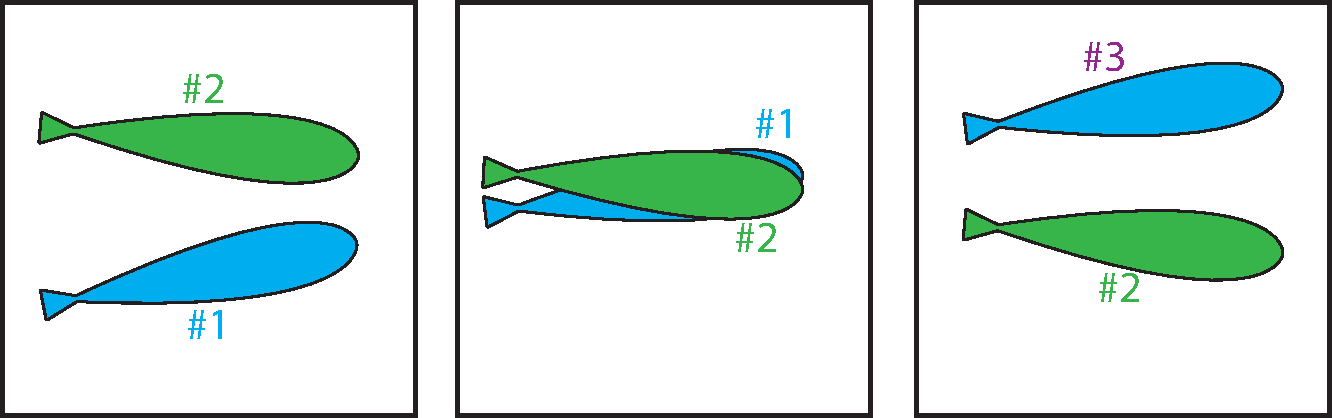
\includegraphics[width=0.9\textwidth]{re_id_ex}
	\caption{Re-ID scenario due to occlusion}
	\label{fig:re-id_Ex}
\end{figure}

\section{Visual Appearance of Zebrafish}

\begin{itemize}
	\item Front vs. sideview (why look at this?)
	\item Maybe an initial test that counts the amounts of general occlusions in a front-view scenario and a side-view scenario
	\item What is an occlusion?
\end{itemize}


Not all occlusions will cause the same types of complications, and some occlusions do not cause any disruption of the trajectory. This is determined by the detection system deployed to track the zebrafish. If the detection of a zebrafish is centred at the head, no occlusion will be detected when the bodies of two zebrafish overlap, however, if detection is done by skeletonisation of the zebrafish, an occlusion will occur (Fig. 2).\\

\begin{figure}[H]
	\centering
	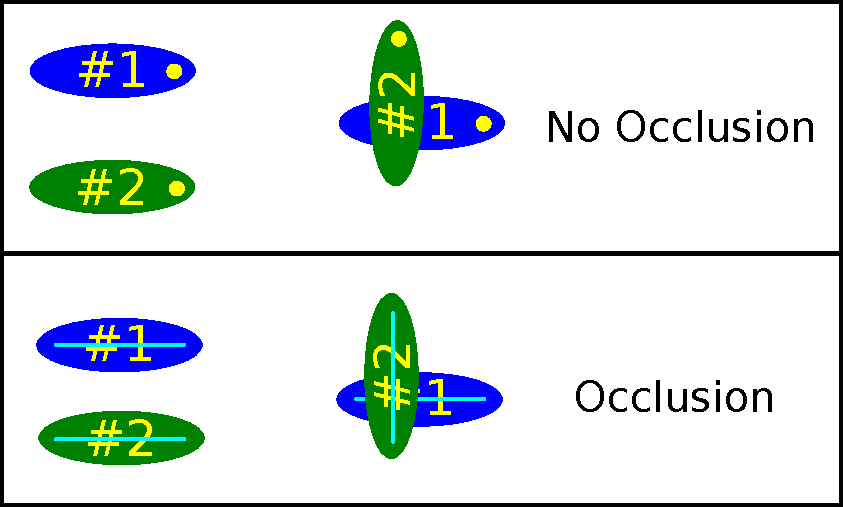
\includegraphics[width=0.85\textwidth]{system_dep_occl}
	\caption{Different types of detection leads to different types of occlusion}
	\label{fig:system_dep_occl}
\end{figure}

A solution to missing tracking data due to occlusions, is to re-link parts of the trajectories (tracklets) to create complete trajectories. This can be done by computing a state vector for each zebrafish and using a Kalman filter which makes predictions of the fish’s position, and thereby estimate what ID belongs to the different zebrafish after an occlusion \citep{Feijo2018, Qian2014}.

\section{Tracking of Zebrafish}

\begin{itemize}
	\item General setup - aquarium, camera, recordings
	\item Automated or manual annotations - what is trajectories
	\item Tracking requires? - What kinds of detection
	\item More fish, leads to occlusions
	\item Occlusion occurred, now what? - Manual vs automated
	\item Predictions - how is it done?	
\end{itemize}

To avoid patching in missing data, another more feasible solution could be made to solve occlusions before they occur by detecting the zebrafish in each frame. Both \cite{Romero-Ferrero2019} and \cite{Dolado2014} propose solutions which detect occlusions in an effort to solve them using computer vision. \cite{Dolado2014} has categorised occlusion types by how the zebrafish overlap each other in an effort to specify the solution. However, the only way they solve the occlusions are through a two-step trial and error process i.e. if the first step does not solve the solution, the second step is applied, without factoring in the occlusion type. 
However, a novel approach could be to recognise an occlusion type in order to apply a predefined optimal solution.

\section{Problem Specification}
In order to be able to categorise different occlusions for system, a detection and classification of occlusions is necessary.

To solve this, some preliminary questions are set up:
\begin{itemize}
	\item How do we detect an occlusion in an image?
	\item How can the occlusion be categorised?
	\item Which types of occlusions are the most frequently occurring?
	\item What solution techniques are there? 
	\item What solution techniques Can be applied to each occlusion type?
\end{itemize}